\chapter{Flash Analysis}
\label{chp:Flash_Analysis}

%checklist:
% - introduction (goal)
% - Test setup
% - Proceedings in this chapter

The goal of this chapter is to find a method, capable of obtaining consistent measures of the environment from measured flashes. Additional goals are to achieve this with the shortest flash and with the least complex method as possible.

In this chapter, the platform is set-up as seen in figure \ref{fig:Flashcapturing}. 
D in the figure represents the distance between the device and the reflecting surface (the floor in this case). All measurements presented in this chapter have been made in a darkroom, a room where no lights from outside can enter, so the test result won't get influenced by other illumination sources.
 
The set-up will first be used to get a reasonable understanding of what flashes look like and how settings of the flash generator influence the received flash. Then, several methods of obtaining these information flashes will be presented and compared. This chapter will conclude with a final settings used in the flash generator and an algorithm to obtain a consistent measure of the environment from the received flash.
\begin{figure}
	\centering     %%% not \center
	\label{fig:Flashcapturing}
	\subfigure[Test setup in illuminated environment]{\label{fig:a}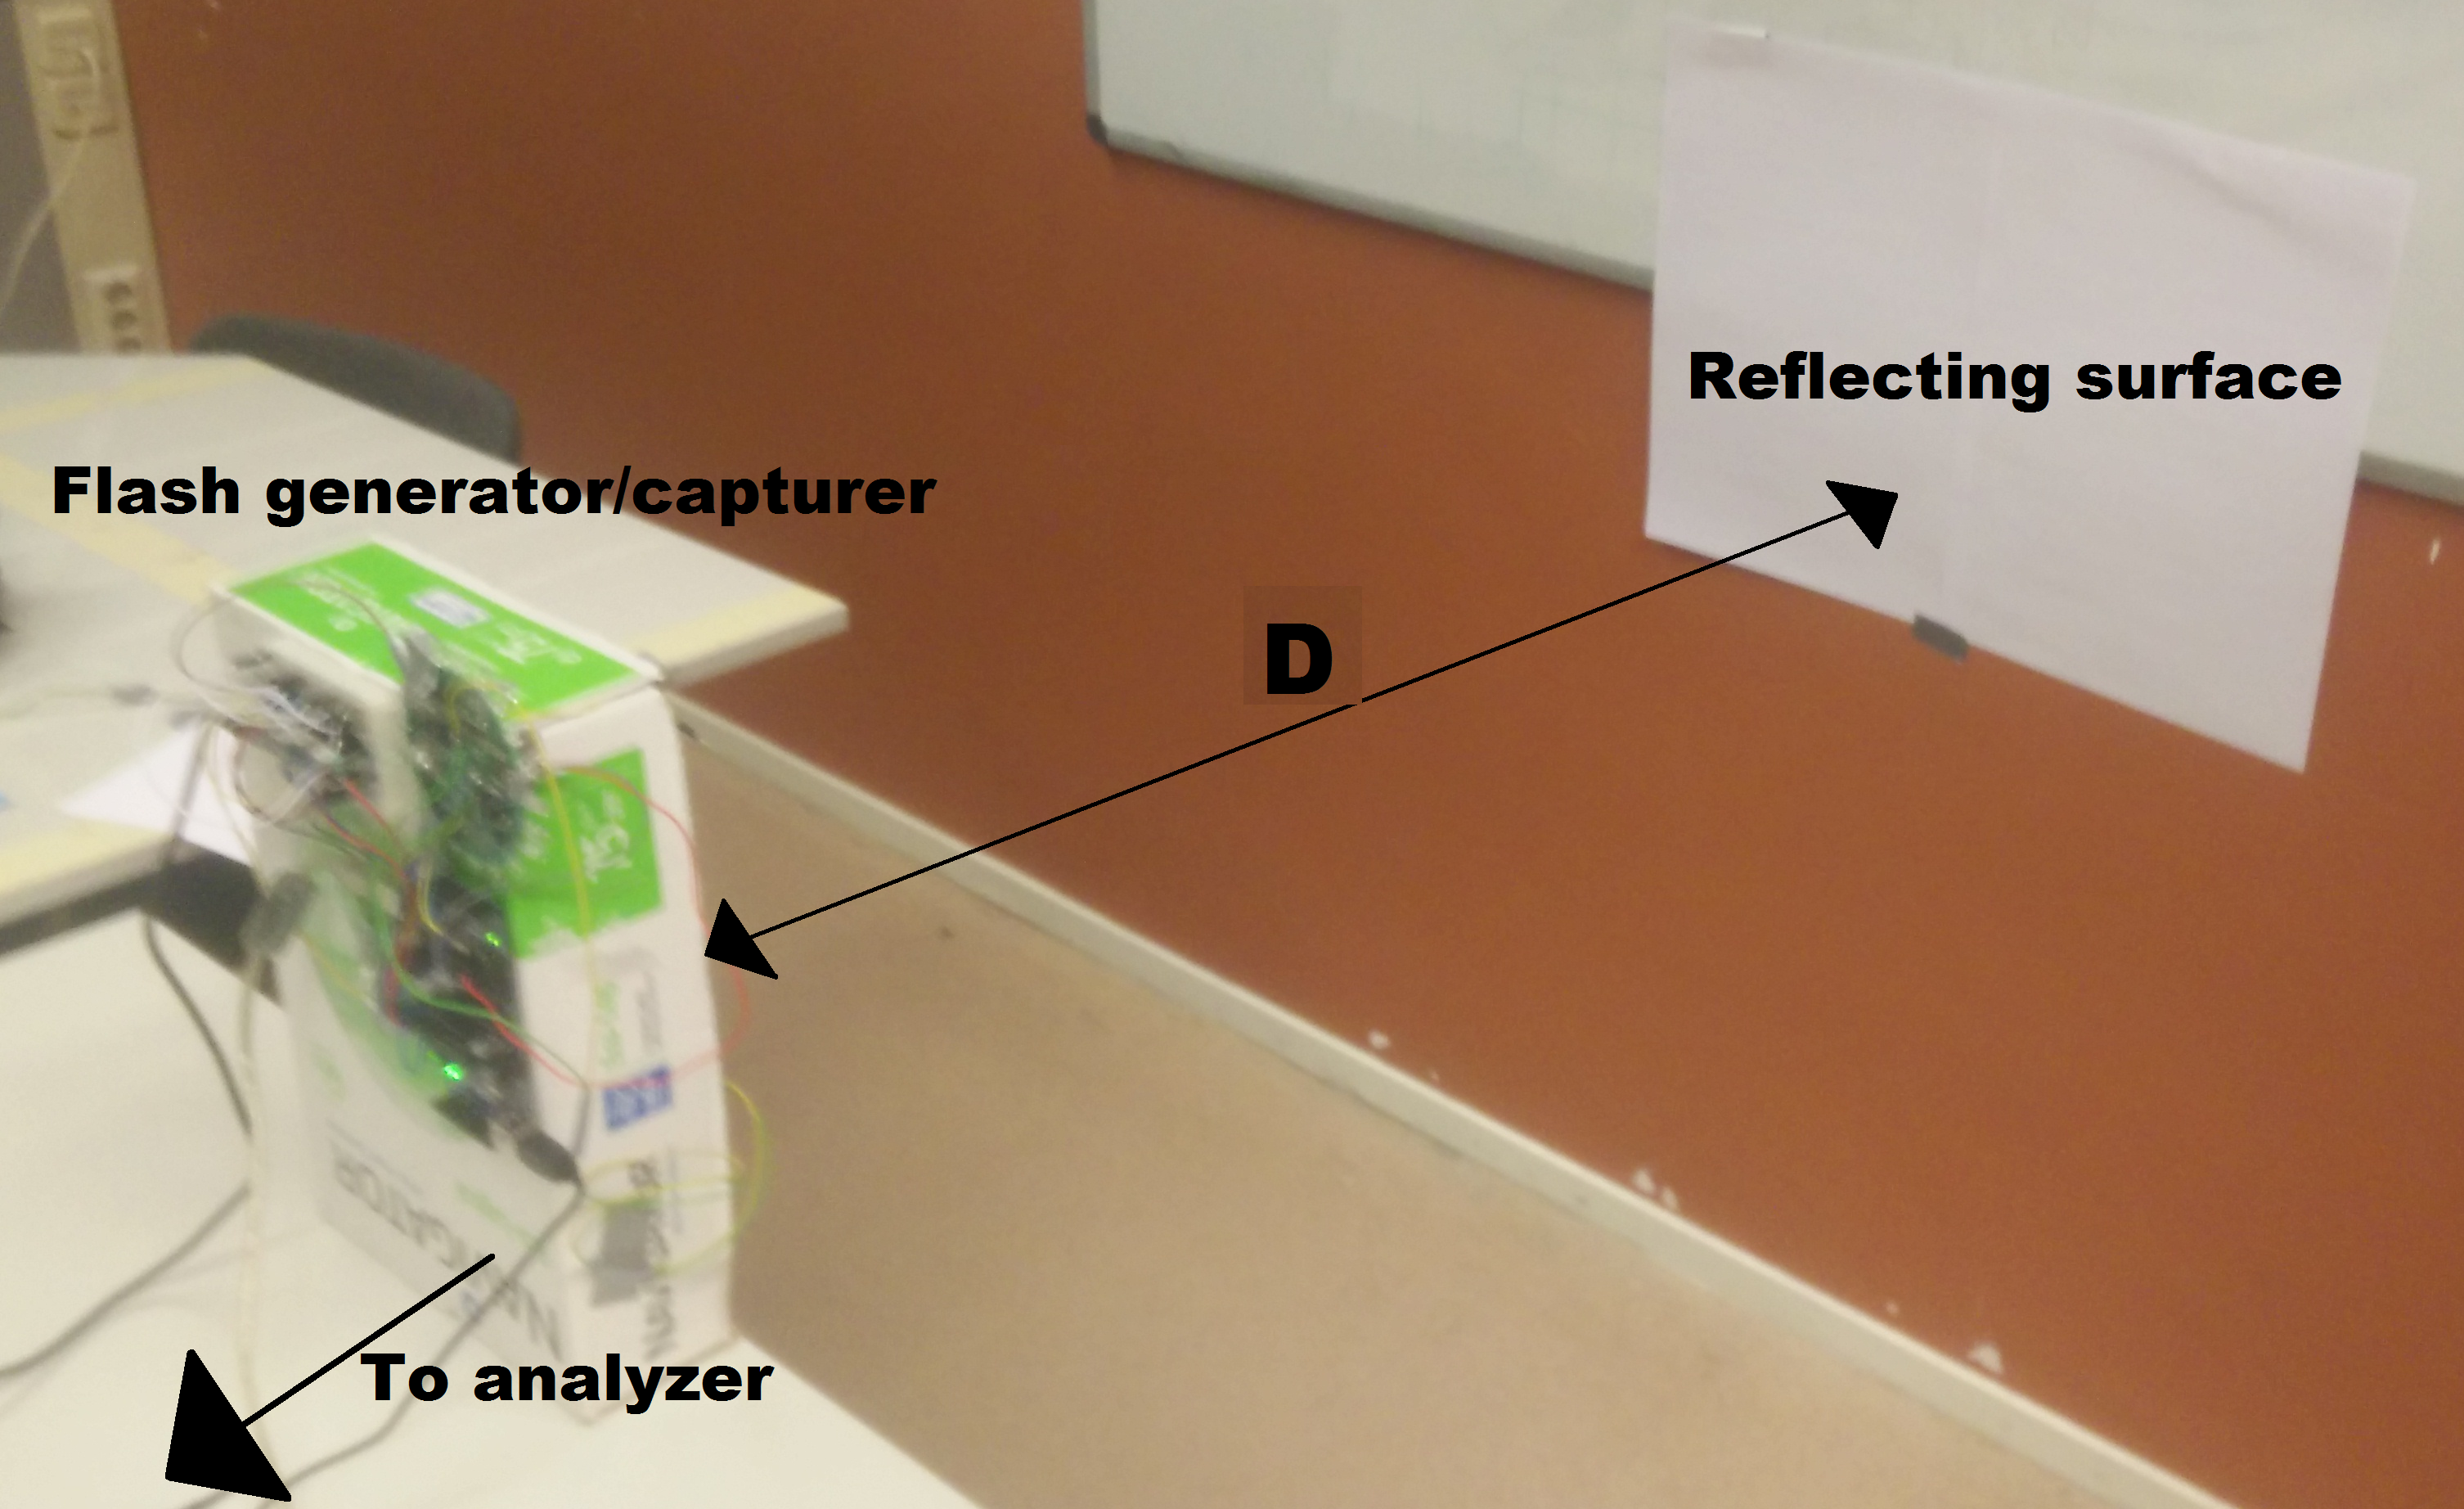
\includegraphics[width=60mm]{pics/Flashcapture_light.png}}
	\subfigure[Test set-up in dark environment]{\label{fig:b}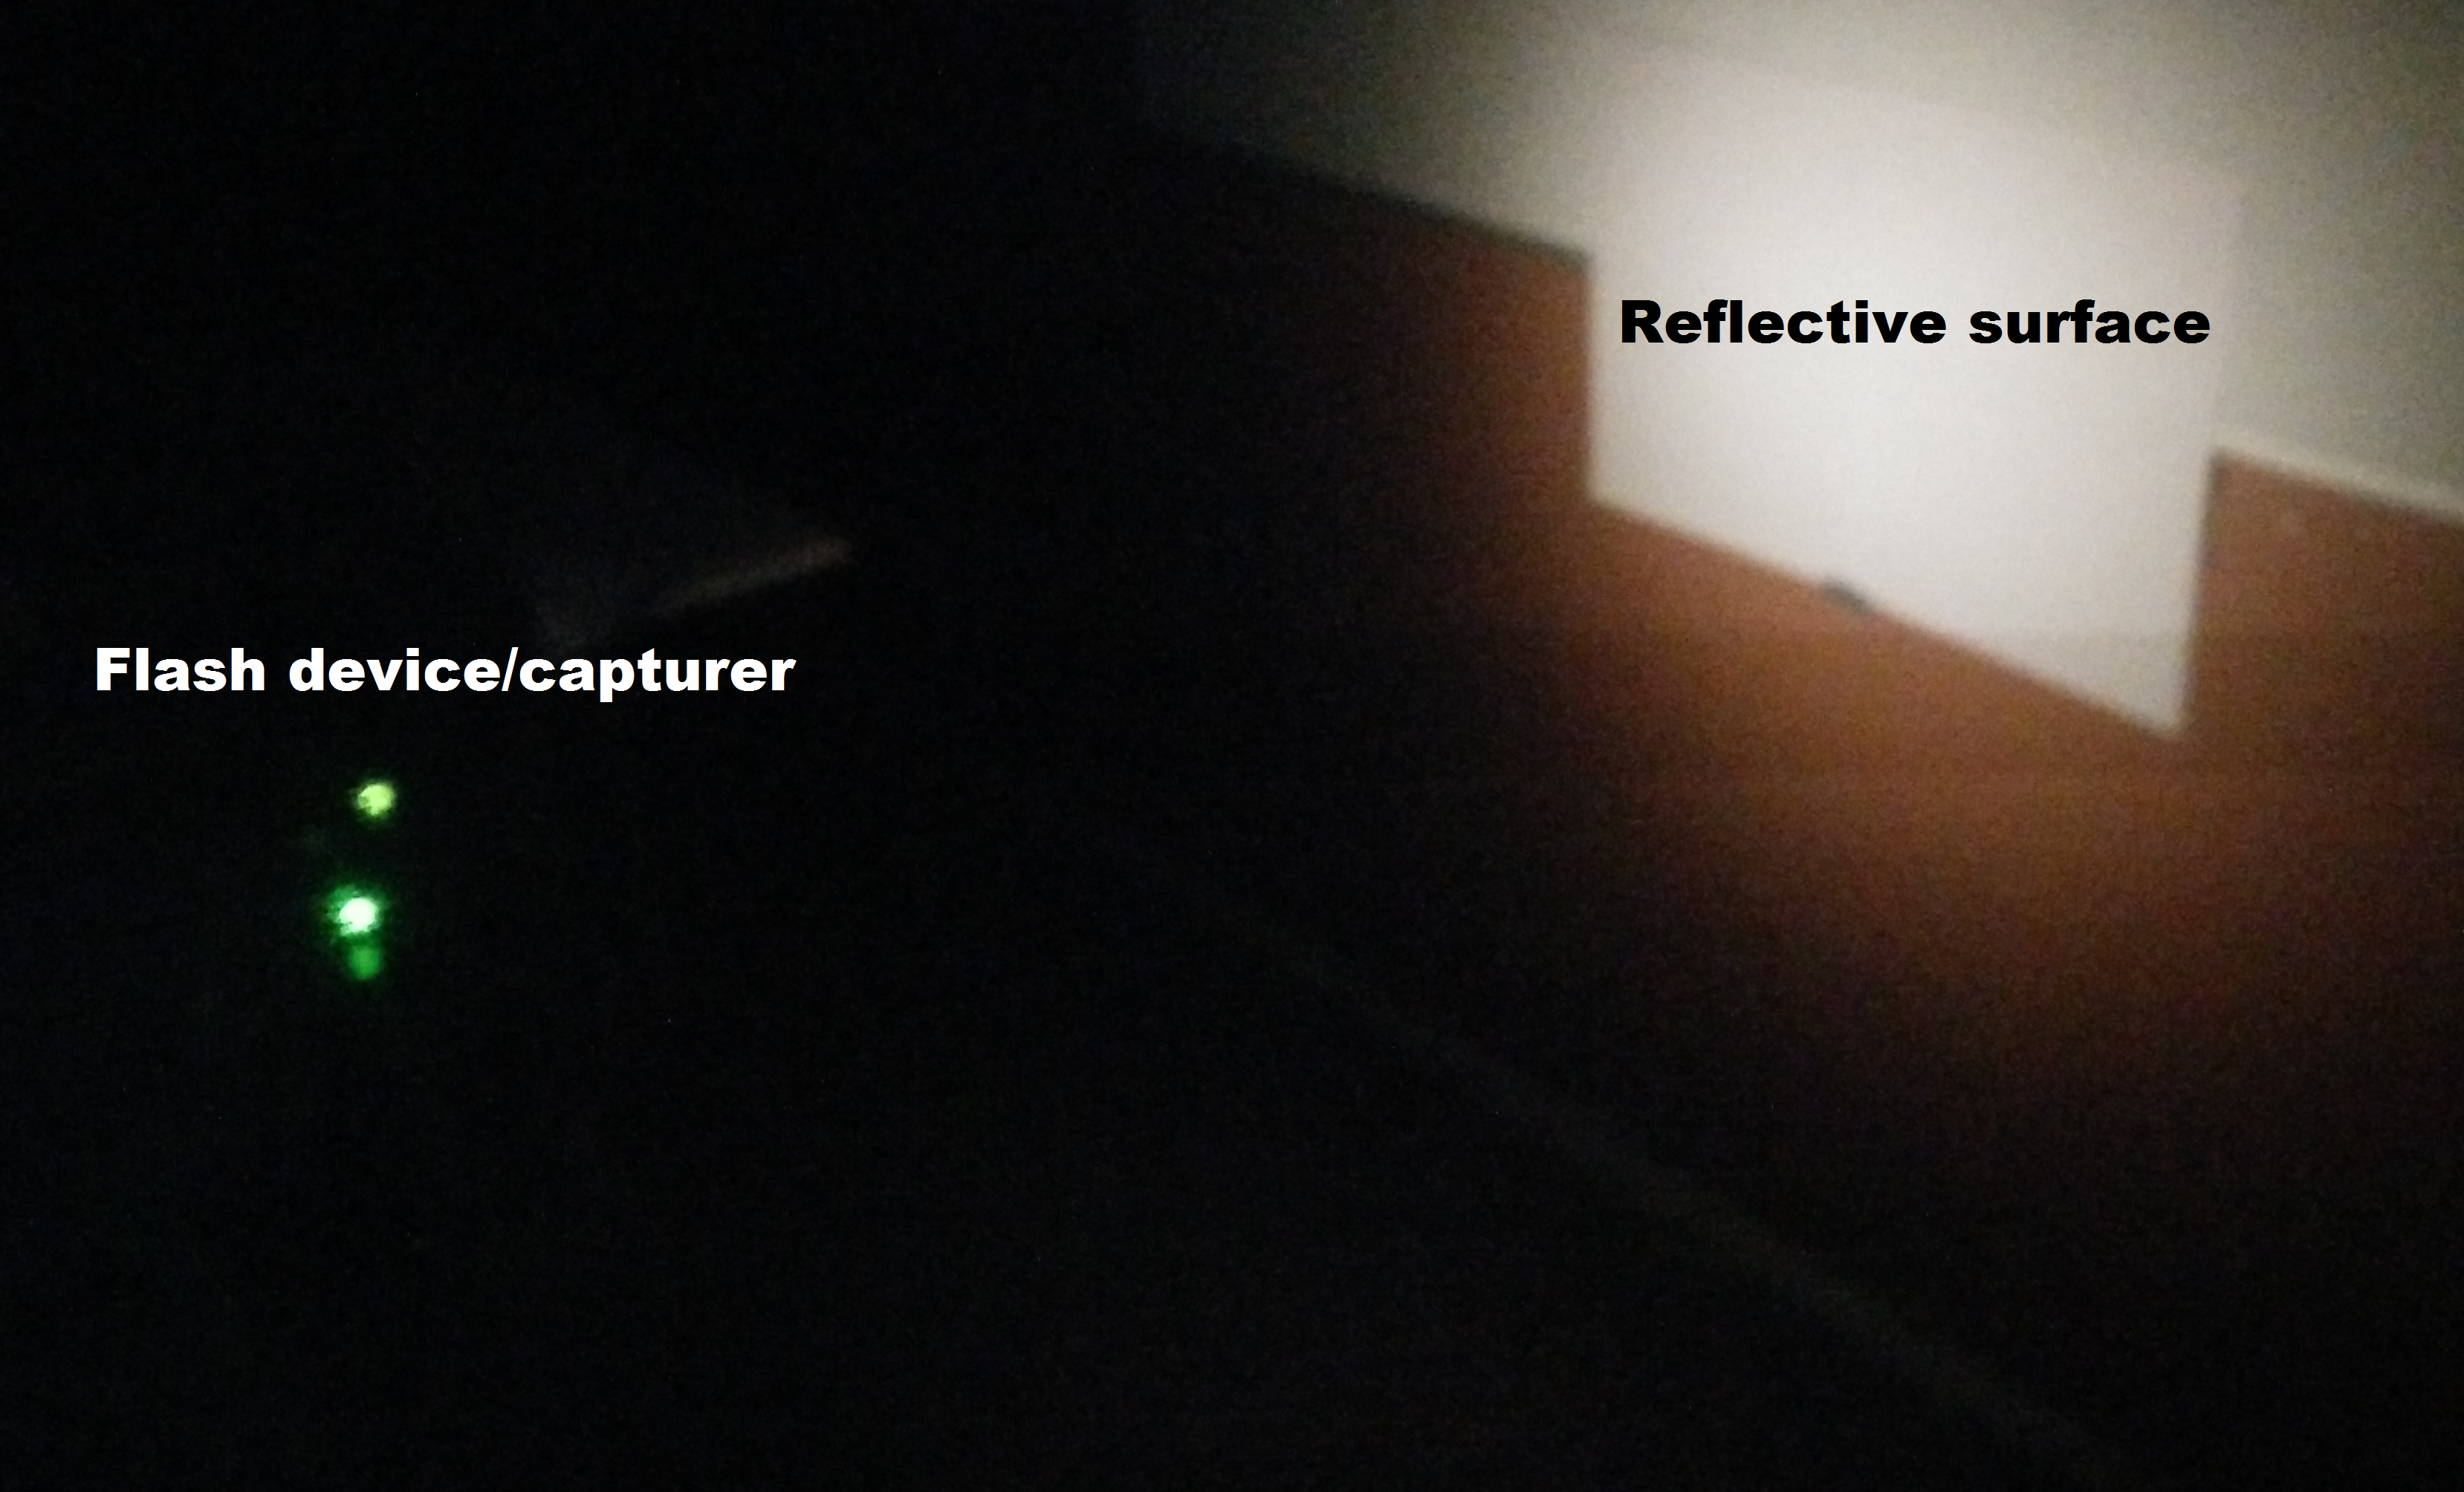
\includegraphics[width=60mm]{pics/Flashcapture_dark.png}}
	\caption{Test set-up used to capture flashes in the darkroom.}
\end{figure}

\section{Flash properties}
\label{sec:Flash_generator}
The test set-up has several parameters which can affect the perceived flash: $T_{on}$ (on time of the LED), $I$ (brightness of the LED), $PD$ (sensitivity of the photo diode) and $D$ (distance between device and reflecting surface). This section shows how each of these parameters influences the received signal. Note that the period, $T$, is not present in the list as should not influence an individual flash, but only the total amount of flashes.

Figure \ref{fig:InfOfTon} shows several responses for different $T_{on}$. In the figure it can be seen that all signals closely match each other, until the light is turned off. This is a useful property as this means it's possible to reduce the $T_{on}$ with no influence on the signal, if the last part is not used.

Figure \ref{fig:InfOfI} shows the influence of using the different amplification circuits of the flash generator. It can be seen that the LED powered with the lower resistance (and thus a higher LED current) is perceived as brighter to the system than the lights powered with a bigger resistor. It's also observed that the LED powered with higher currents show up earlier to the system. This is because LEDs driven with higher currents turn on faster \cite{LED_on}. This means that if a lower LED current is used a bigger $T_on$ is required to obtain useful information.

Figure \ref{fig:InfOfD} shows a set of measured flashes at a variance distance from the wall. It clearly shows that if the distance increases, the observed light also decreases. This is logical, as when light travels longer distances, the relative intensity of the light decreases. 

Figure \ref{fig:InfOfD} displays what happens to the signal if it's sampled by different photo diodes (with a different amplification circuit). As would be expected, the signal with the bigger amplification perceives the signal to be several times stronger. It's however important to note that the frequency ripple on the signal is significantly lower with the strong amplifier. This makes sense as using a higher resistance in the amplification circuit (resulting in a higher gain) increases the osculation frequency of the amplifier.

Figure \ref{fig:InfOfPD} shows what happens when the different photo diodes are used. As expected, the RSS rises once we increase the gain on the photo diode. $PD_3$ almost instantly saturates as the gain is too strong when used in combination with $I_1$. $PD_3$ is therefore also displayed with $I_3$. Another thing which changes is the ripple frequency. This is expected, as the resistor in the feedback loop of the amplifier was changed.


\begin{figure}
	\centering     %%% not \center
	\label{fig:InfOf}
	\subfigure[]{\label{fig:InfOfTon}\includegraphics[width=60mm]{pics/InfluenceOfTon.png}}
	\subfigure[]{\label{fig:InfOfI}\includegraphics[width=60mm]{pics/InfluenceOfI.png}}
	\\
	\subfigure[]{\label{fig:InfOfD}\includegraphics[width=60mm]{pics/InfluenceOfD.png}}
	\subfigure[]{\label{fig:InfOfPD}\includegraphics[width=60mm]{pics/InfluenceOfPD.png}}
	\caption{Several perceived flashes generated with different settings of $T_{on}$, $I_{LED}$, $D$ and $PD$.}
\end{figure}

% properites checklist:
% - What happens if distance increases
%   + fig with multiple distances
% - What happens if t-on time increases
%   + fig with increasing t-on
% - What happens if intensity increases
%   + fig multiple 3 intensities
% sumarize in table 
% conclude:
% - 

\section{Flash features}
This section explores what kind of features can be extracted from a flash signal. It will then compare the methods based on required $T_{on}$, precision, the "Signal to Noise Ratio" (SNR) and computational complexity.

\subsection{Feature considerations}
The maximum of a flash response could contain useful information. Even though the light at the first maximum has not fully turned on yet, it still is some measure of the perceived light. This can be especially useful if the maximum of the flash always occurs at the exact same moment in time relative to the light turning on. If that is the case, then the maximum value of the first peak could provide us with enough information of the environment. If the maximum value of the first peak holds enough information, then a very small $T_{on}$ can be used to obtain this value, as decreasing $T_{on}$ does not significantly influence the height and form of the first peak.

Another possibility is the to remove the oscillation of the signal with a low pass filter and then take the maximum value of the filtered signal. This method less reliant on precise timing of the pulse. It also uses more samples of the signal and should therefore be able to obtain a value which better represents the reflections of the current environment than the maximum method. A downside to this method is that a filter designed to deal with one frequency of ripple, is not immediately suited to deal with the other possible ripple frequency.

Another method considered is to use the surface underneath the signal. This method has the advantage of being both simple and flexible. It does not matter if $T_{on}$ is chosen big or small. It also does not care about the ripple frequency of the amplifier This method simply sums all information available to obtain a measure of the reflections.

The final possibility considered is the filtered sum method. It first uses a filter to smooth the signal to then calculated the surface underneath it. It also requires multiple filters to be designed (one for each $PD$ amplifier). It might however give a more detailed result than the filter method, as more information is used obtaining the data point.

\subsection{Feature comparison}
A test was created to compare the effectiveness of each feature with various settings in a full scale environment ($D = 280cm$). The test was executed as follows:
\begin{enumerate}[itemsep=-1ex]
	\item Set the parameters for the given test ($PD$, $I$, $T_on$).
	\item Move a highly reflective piece of cloth underneath the set-up at $185cm$ ($D = 95cm$).
	\item Move the piece of cloth underneath the setup again, but no from the other direction.
	\item Calculate the SNR of the received signal.
\end{enumerate}
If we refere to the 'SNR' in this thesis we mean the SNR as defined in equation \ref{eq:snr}. This equation calculates ratio between the standard deviation of the signal when noting is passing by and the absolute minimum and maximum of when something is. The higher the SNR, the easier it should be to distinguish between activity and no activity later on.

\begin{equation}
SNR(PD) = \left(\frac{\mu(PD_{NoEvent}) - min(PD_{event})}{\sigma(PD_{NoEvent})} + \frac{ max(PD_{event}) - \mu(PD_{NoEvent})}{\sigma(PD_{NoEvent})}\right)
\end{equation}
\begin{equation}
\label{eq:snr}
SNR(PD) = \frac{max(PD_{Event}) - min(PD_{Event})}{\sigma(PD_{NoEvent})} 
\end{equation}

The test was done with all combinations of $PD$ and $I$. Only the combinations of $PD_2, I_{1}$ and $PD3, I_{3}$ gave potential usable results at full scale as for other combinations the flash was invisible or or too bright (saturation). Several consecutive captured features can be seen in the Figures \ref{fig:SimpleFeatures} and \ref{fig:complexFeatures}. These where then used to calculated the SNR for each scenario. 

An overview of all calculated SNR values can be seen in table \ref{SNR_results}. 

\begin{table}[]
	\centering
	\label{SNR_results}
\begin{tabular}{l|lll|lll|}
	& \multicolumn{3}{c|}{SNR: $PD_2, I_1$} & \multicolumn{3}{c|}{SNR: $PD_3, I_3$} \\
	$T_{on}$         & $150 \mu s$ & $200\mu s$ & $250\mu s$ & $150\mu s$  & $20\mu s$  & $25\mu s$  \\ \hline
	Maximum          & 35          & 38         & 40         & 5           & 5          & 5          \\
	Filtered maximum & 39          & 65         & 66         & 20          & 27         & 33         \\
	Sum              & 45          & 75         & 95         & 18          & 20         & 26         \\
	Filtered sum     & 50          & 105        & 100        & 19          & 20         & 24        
\end{tabular}
	\caption{Overview of the test results}
\end{table}




\begin{figure}
	\centering     %%% not \center
	\label{fig:SimpleFeatures}
	\subfigure[]{\label{fig:simple_PD2}\includegraphics[width=60mm]{pics/SNR_simple_PD2.png}}
	\subfigure[]{\label{fig:simple_PD3}\includegraphics[width=60mm]{pics/SNR_simple_PD3.png}}
	\caption{Data extracted using the maximum and filtered maximum methods with $T_{on} = 250\mu s$.}
\end{figure}

\begin{figure}
	\centering     %%% not \center
	\label{fig:complexFeatures}
	\subfigure[]{\label{fig:complex_PD2}\includegraphics[width=60mm]{pics/SNR_complex_PD2.png}}
	\subfigure[]{\label{fig:complex_PD3}\includegraphics[width=60mm]{pics/SNR_complex_PD3.png}}
	\caption{Data extracted using the sum and filtered sum method with $T_{on} = 200\mu s$.}
\end{figure}

\begin{table}[]
	\hskip-2.0cm
	\label{tbl:FlashAnalyserResults}
\begin{tabular}{l|lll|lll|ll}
	& \multicolumn{3}{c|}{$PD_2, I_1$} & \multicolumn{3}{c|}{$PD_3, I_3$} & \multicolumn{1}{c}{\multirow{2}{*}{\begin{tabular}[c]{@{}c@{}}\# of\\ Additions\end{tabular}}} & \multicolumn{1}{c}{\multirow{2}{*}{\begin{tabular}[c]{@{}c@{}}\# of\\ Multiplications\end{tabular}}} \\
	Method           & $T_{on}[\mu s]$  & Noise ($\sigma$) & SNR  & $T_{on}[\mu s]$  & Noise ($\sigma$) & SNR  & \multicolumn{1}{c}{}                                                                           & \multicolumn{1}{c}{}                                                                                 \\ \hline
	Maximum          & 15               & 1.9    & 5    & 20               & 18.8   & 40   & N                                                                                              & -                                                                                                    \\
	Filtered maximum & 25               & 8.4    & 33   & 25               & 6.5    & 65   & N + 4N                                                                                         & 5N                                                                                                   \\
	Sum              & 25               & 450    & 26   & 25               & 192    & 95   & N                                                                                              & -                                                                                                    \\
	Filtered sum     & 25               & 424    & 23   & 20               & 142    & 100  & N + 4N                                                                                         & 5N                                                                                                  
\end{tabular}
	\caption{Overview of the best found settings to extract each feature.}
\end{table}
% - Compare explored methods on and SNR (std vs max std of mean), Energy used (required t-on),
% - Choose method
% - Choose sample reuqency



The final parameter to decide is the period of the signal, $T$. This value has no influence on the noise measured on the signal except for the frequency. It has however a clear influence on how much light is used by the system, as decreasing $T$ directly increases the amount of flashes. We can't choose a too low value for $T$ as then users will observe flickering of the light. Another reason $T$ can't be chosen too low is that certain kind of noise still needs to be filtered out of the system. It is almost guaranteed that some 50Hz component will be seen in the signal, as long as its connected to the net. 

For these reasons, $T$ was chosen to be 800$\mu s$. This value results in a flash frequency of 125Hz. This value is more that the Nyquist frequency of the 50Hz. Even though literature recommends at least 200Hz to prevent the visibility of flickering, none was observed by 10 different test subjects with this setting of $T$. Another benefit is that the found method does not require a lot of computational power.

\section{Conclusion}
The Flash analyser will run at a frequency of 125Hz, a $T_on$ of $200\mu s$ with maximum light intensity $I_1$. These settings provide a reasonable level of precision for the full scale scenario. The next step for the project is creating an algorithm for the analyser, capable of analysing a set of consecutive flashes.